\documentclass[11pt,a4paper]{article}
\usepackage[T1]{fontenc}
\usepackage[margin=20mm]{geometry}
\usepackage{amsmath}
\usepackage{array,booktabs}
\usepackage{enumitem}
\usepackage{listings}
\usepackage{tikz}
\usetikzlibrary{arrows.meta,positioning,calc}
\usepackage{hyperref}
\hypersetup{hidelinks,pdftitle={Digital System Design -- Spring 2009 Final Exam}}
\setlength{\parindent}{0pt}
\setlength{\parskip}{6pt}
\setlist[enumerate]{leftmargin=2em,itemsep=4pt,topsep=4pt}
\lstset{language=Verilog,basicstyle=\ttfamily\small,columns=fullflexible,
  keepspaces=true,showstringspaces=false,frame=single,breaklines=true,
  aboveskip=5pt,belowskip=5pt}
\newcommand{\question}[2]{\subsection*{Question #1\hfill\normalfont #2}}
\begin{document}
\begin{center}
  {\LARGE\bfseries Digital System Design}\\[5pt]
  {\large Final Exam (96/06/15)\\Spring 2009}\\[5pt]
  Total points: 105 points
\end{center}
\begin{quote}\small
\textbf{Transcription and provenance.} Source: \texttt{Final-Exam-2009.pdf}.
The year and date above are copied as printed; their inconsistency is not
resolved here. All five question statements and their scores are retained.
The circuit is redrawn semantically with editable TikZ. The timing diagram
is expressed as an editable interval table retaining every visible input
value. The numbered instructions below are quoted exam content; bracketed
notes identify editorial observations. No solution assumptions are added.
\end{quote}

\question{1}{15\%}
Correct the errors of the following Verilog codes.
\begin{lstlisting}
module CheerUp (AndYou, IamFine, VeryGood, NotBad, Sel);
    output [1:0] IamFine, AndYou;
    input [1:0] VeryGood, NotBad;
    reg [1:0] VeryGood, NotBad;
    input Sel;
    reg [1:0] IamFine;

    // continue in the right hand side.
    AndYou = VeryGood | NotBad;

    always @(Sel or VeryGood)
        IamFine[0] = Sel ? VeryGood[0] : VeryGood[1];
        IamFine[1] = Sel ? NotBad[0] : NotBad[1];
endmodule
\end{lstlisting}
{\small [Editorial note: the two printed columns are joined above. The errors,
including the missing block delimiters, are preserved for the exercise.]}

\question{2}{10\%}
Please state what kind of hardware is inferred? Draw its symbol.
(For example: AND gate, OR gate, \ldots)
\begin{enumerate}[label=(\alph*)]
\item
\begin{lstlisting}
reg outsig;
always @(en or ina)
    if (en) outsig = ina;
\end{lstlisting}
\item
\begin{lstlisting}
reg outsig;
always @(en or ina)
    if (en) outsig = ina;
    else outsig = 1'bz;
\end{lstlisting}
\end{enumerate}

\newpage
\question{3}{45\%}
Write the Verilog code of the following modules.
\begin{enumerate}[label=(\alph*)]
\item A 16-bit 2-to-1 multiplexer. (10\%)
\begin{lstlisting}
module MUX21(ina, inb, sel, out);
    ...
endmodule
\end{lstlisting}

\item A 16-bit positive-edge-triggered D flip-flop with asynchronous reset.
(10\%)
\begin{lstlisting}
module DFF16(Q, D, clk, rst);
    ...
endmodule
\end{lstlisting}

\item A 16-bit logic shifter whose function is defined as the following
table. Note that you cannot use \texttt{<<} or \texttt{>>} operators. (10\%)
\begin{center}
\begin{tabular}{c l l}
\toprule
LR & Output & Description\\
\midrule
0 & \texttt{ShOut = C >> 1} & Logic shift to the right by 1 bit\\
1 & \texttt{ShOut = C << 1} & Logic shift to the left by 1 bit\\
\bottomrule
\end{tabular}
\end{center}
\begin{lstlisting}
module Shifter(ShOut, C, LR);
    ...
endmodule
\end{lstlisting}

\item A 16-bit arithmetic logic unit (ALU) having the following functions.
(15\%)
\begin{center}
\begin{tabular}{c l l}
\toprule
CTR & Output & Description\\
\midrule
0 & \texttt{ALUOut = A + B} & Addition\\
1 & \texttt{ALUOut = A - B} & Subtraction\\
2 & \texttt{ALUOut = A + 1} & Increase by 1\\
3 & \texttt{ALUOut = A - 1} & Decrease by 1\\
\bottomrule
\end{tabular}
\end{center}
\begin{lstlisting}
module ALU(ALUOut, A, B, CTR);
    ...
endmodule
\end{lstlisting}
\end{enumerate}
{\small [Editorial note: the original does not specify MUX selection polarity,
reset polarity or reset value. A worked implementation must state its choices
separately.]}

\newpage
\question{4}{20\%}
Connect those instances in Question 2 as the following figures. Note that
all the data paths are 16 bits.

{\small [Editorial note: ``Question 2'' is the original reference. The named
MUX, DFF, ALU and Shifter modules are in Question 3.]}

\begin{center}
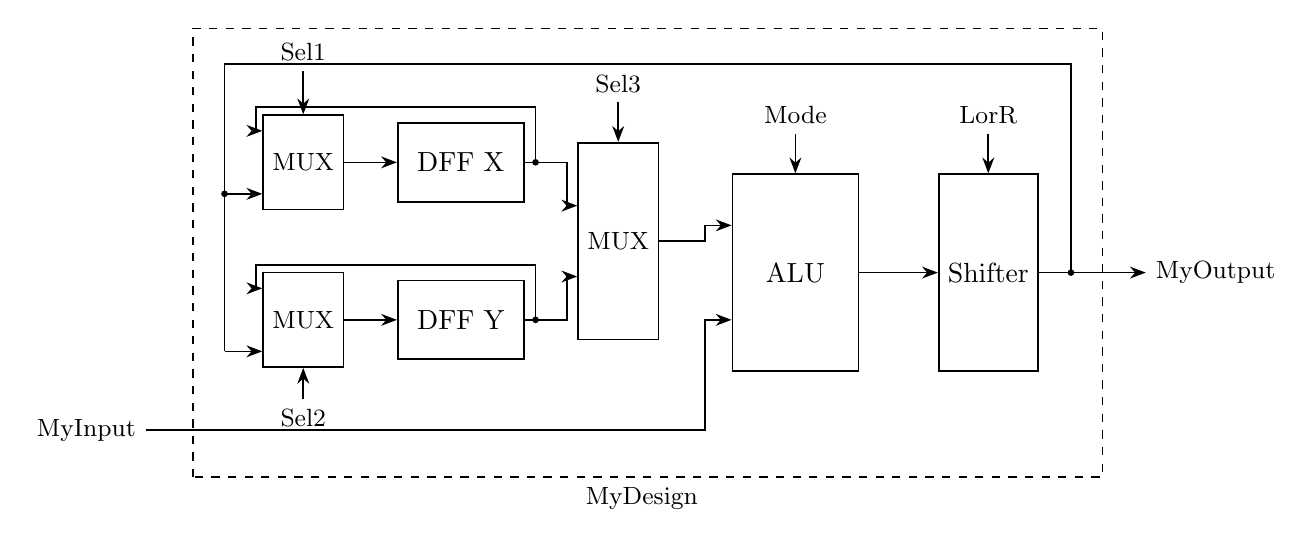
\begin{tikzpicture}[x=1cm,y=1cm,>=Stealth,semithick,
  box/.style={draw,minimum width=16mm,minimum height=10mm,align=center},
  mux/.style={draw,minimum width=8mm,minimum height=12mm,align=center,font=\small},
  lab/.style={font=\small}, data/.style={->}]
  \draw[dashed] (0.6,0.4) rectangle (12.15,6.1);
  \node[lab,anchor=north] at (6.3,0.4) {MyDesign};
  \node[mux] (mx) at (2.0,4.4) {MUX};
  \node[mux] (my) at (2.0,2.4) {MUX};
  \node[box] (dx) at (4.0,4.4) {DFF X};
  \node[box] (dy) at (4.0,2.4) {DFF Y};
  \node[mux,minimum height=25mm] (ma) at (6.0,3.4) {MUX};
  \node[box,minimum height=25mm] (alu) at (8.25,3.0) {ALU};
  \node[box,minimum width=12mm,minimum height=25mm] (sh) at (10.7,3.0) {Shifter};
  \draw[data] (mx.east) -- (dx.west);
  \draw[data] (my.east) -- (dy.west);
  \draw[data] (dx.east) -- (5.35,4.4) -- (5.35,3.85) -- (ma.west |- {5.35,3.85});
  \draw[data] (dy.east) -- (5.35,2.4) -- (5.35,2.95) -- (ma.west |- {5.35,2.95});
  \draw[data] (ma.east) -- (7.1,3.4) -- (7.1,3.6) -- (alu.west |- {7.1,3.6});
  \draw[data] (alu.east) -- (sh.west);
  \draw[data] (sh.east) -- (12.7,3.0) node[lab,right] {MyOutput};
  \draw (11.75,3.0) -- (11.75,5.65) -- (1.0,5.65) -- (1.0,2.0);
  \fill (11.75,3.0) circle (1.2pt);
  \draw[data] (1.0,4.0) -- (mx.west |- {1.0,4.0});
  \draw[data] (1.0,2.0) -- (my.west |- {1.0,2.0});
  \fill (1.0,4.0) circle (1.2pt);
  \draw[data] (4.95,4.4) -- (4.95,5.1) -- (1.4,5.1) -- (1.4,4.8) -- (mx.west |- {1.4,4.8});
  \fill (4.95,4.4) circle (1.2pt);
  \draw[data] (4.95,2.4) -- (4.95,3.1) -- (1.4,3.1) -- (1.4,2.8) -- (my.west |- {1.4,2.8});
  \fill (4.95,2.4) circle (1.2pt);
  \draw[data] (0.0,1.0) node[lab,left] {MyInput} -- (7.1,1.0) -- (7.1,2.4) -- (alu.west |- {7.1,2.4});
  \draw[data] (mx.north)+(0,0.55) node[lab,above] {Sel1} -- (mx.north);
  \draw[data] (my.south)+(0,-0.4) node[lab,below] {Sel2} -- (my.south);
  \draw[data] (ma.north)+(0,0.5) node[lab,above] {Sel3} -- (ma.north);
  \draw[data] (alu.north)+(0,0.5) node[lab,above] {Mode} -- (alu.north);
  \draw[data] (sh.north)+(0,0.5) node[lab,above] {LorR} -- (sh.north);
\end{tikzpicture}
\end{center}
{\small [Figure note: each register-input MUX receives its own register output
at the upper input and the common MyOutput feedback at the lower input.
The central MUX receives X above and Y below. CLK and reset wiring and input
port/polarity labels are absent from the source figure. The diagram therefore
does not assign \texttt{ina}/\texttt{inb} or a selection polarity.]}

\question{5}{15\%}
Write test bench to test the above module called ``MyDesign'' as the following
timing diagram.

\textbf{Timing diagram, expressed as intervals.} The original marks a
20 ns clock period. Taking the first dashed vertical line as $t=0$, CLK is
high on $[20k,20k+10)$ ns and low on $[20k+10,20k+20)$ ns for $k=0,\ldots,4$.
The five complete periods and input values shown are:
\begin{center}
\small
\begin{tabular}{c c c c c c l}
\toprule
Time (ns) & Sel1 & Sel2 & Sel3 & LorR & Mode & MyInput\\
\midrule
$[0,20)$   & 0 & 1 & 1 & 0 & \texttt{2'b00} & \texttt{16'h1a}\\
$[20,40)$  & 1 & 1 & 1 & 0 & \texttt{2'b00} & \texttt{16'hea}\\
$[40,60)$  & 1 & 0 & 0 & 0 & \texttt{2'b01} & \texttt{16'h55}\\
$[60,80)$  & 0 & 0 & 0 & 1 & \texttt{2'b10} & \texttt{16'h8c}\\
$[80,100)$ & 0 & 0 & 0 & 1 & \texttt{2'b11} & \texttt{16'hff}\\
\bottomrule
\end{tabular}
\end{center}
{\small [Editorial note: Sel2 and Sel3 share a single trace in the original.
The source has no reset waveform, initial register values, output waveform,
or simulator scheduling convention for inputs changing at clock edges.
The displayed endpoint at 100 ns does not specify a subsequent full interval.]}
\end{document}
